\section{Рабочий проект}
\subsection{Классы, используемые при разработке приложения}

Можно выделить следующий список классов и их методов, использованных при разработке приложения (таблица \ref{class:table}). 

\renewcommand{\arraystretch}{0.8} % уменьшение расстояний до сетки таблицы
\begin{xltabular}{\textwidth}{|X|p{2.5cm}|>{\setlength{\baselineskip}{0.7\baselineskip}}p{4.85cm}|>{\setlength{\baselineskip}{0.7\baselineskip}}p{4.85cm}|}
	\caption{Описание классов, используемых в приложении\label{class:table}}\\
	\hline \centrow \setlength{\baselineskip}{0.7\baselineskip} Название класса & \centrow \setlength{\baselineskip}{0.7\baselineskip} Модуль, к которому относится класс & \centrow Описание класса & \centrow Методы \\
	\hline \centrow 1 & \centrow 2 & \centrow 3 & \centrow 4\\ \hline
	\endfirsthead
	\caption*{Продолжение таблицы \ref{class:table}}\\
	\hline \centrow 1 & \centrow 2 & \centrow 3 & \centrow 4\\ \hline
	\finishhead
	MainWindow & Главный модуль & MainWindow – главный класс приложения. Содержит основные функции для создания и взаимодействия с рабочей областью. & create\_root(self, cwidth, cheight, fo, sImg)
	Cоздает основное окно, которое состоит из меню и канваса
	paint(event, self)
	Отрисовывает круги в месте клика мышки
	brelease(event, self)
	Очищает созданные списки
	cr\_line(event, self)
	Соединяет два отрисованных круга линией\\
	\hline 
	FirstWindow & Доп. модуль & FirstWindow – класс, создающий начальное окно с вводом параметров изображения. & firstroot(self)
	Создает начальное окно 
	check\_var(self)
	Проверяет значение вводимых переменных
	create\_newImg(self)
	Уничтожает начальное окно и вызывает функцию для создания основного\\
	\hline
	Inter & Доп. модуль & Inter – класс, отвечающий за сохранение и открытие других изображений. & save\_img(self)
	Сохраняет изображение
	open\_img(self)
	Открывает изображение
	createImg(self)
	Вызывает начальное окно
	w\_and\_h(self, fname)
	Узнает размеры, открываемого изображения\\
	\hline
	Brush & Доп. модуль & Brush – класс, отвечающий за параметры кисти. & eraser(self)
	Меняет цвет кисти на белый
	size\_change(self, new\_size)
	Меняет радиус кисти на выбранный
	color\_change(self)
	Меняет цвет кисти на выбранный
	clear\_canvas(self, f)
	Полностью очищает canvas
	pour(self, f)
	Полностью очищает canvas, устанавливает фон с таким же цветом, как и у кисти
	brush(self)
	Выбирает режим обычного рисования
	pixel\_brush(self)
	Выбирает режим пиксельного рисования
	eraser(self)
	Меняет цвет кисти на белый \\
	\hline
\end{xltabular}
\renewcommand{\arraystretch}{1.0} % восстановление сетки

\subsection{Системное тестирование разработанного приложения}

На рисунке \ref{osn:image} представлено основное окно графического редактора.
\newpage % при необходимости можно переносить рисунок на новую страницу
\begin{figure}[H] % H - рисунок обязательно здесь, или переносится, оставляя пустоту
\center{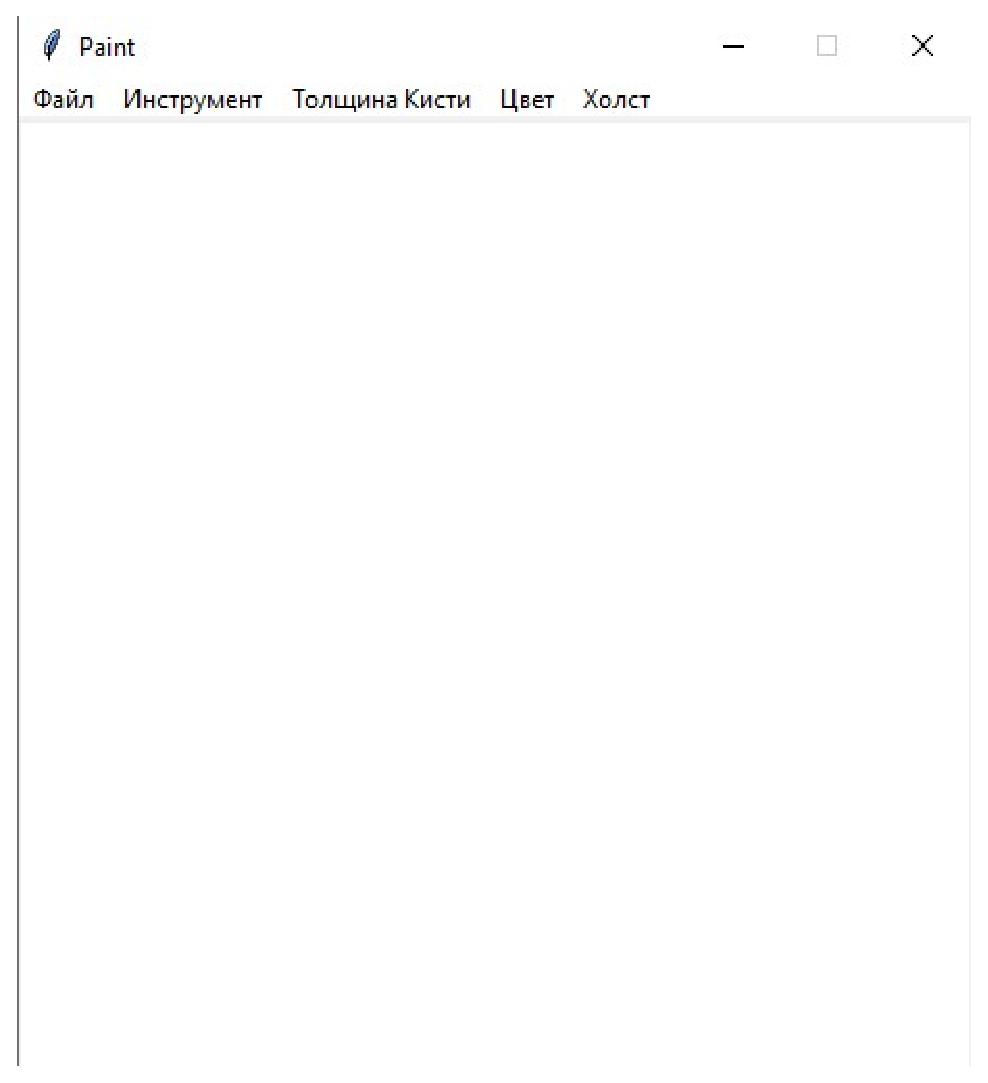
\includegraphics[width=1\linewidth]{osn}}
\caption{Основное окно}
\label{osn:image}
\end{figure}

На рисунке \ref{vvod:image} представлено начальное окно с выбором параметров будущего изображения.

\begin{figure}[H]
\center{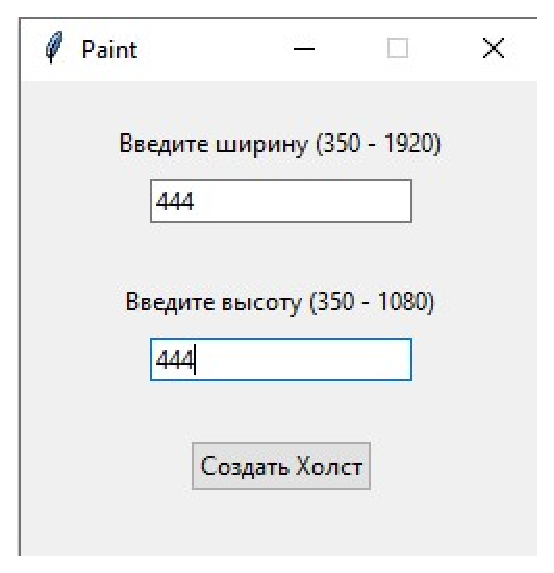
\includegraphics[width=1\linewidth]{vvod}}
\caption{Начальное окно}
\label{vvod:image}
\end{figure}

На рисунке \ref{sve:image} представлено сохранение файла через диалоговое окно.

\begin{figure}[H]
\center{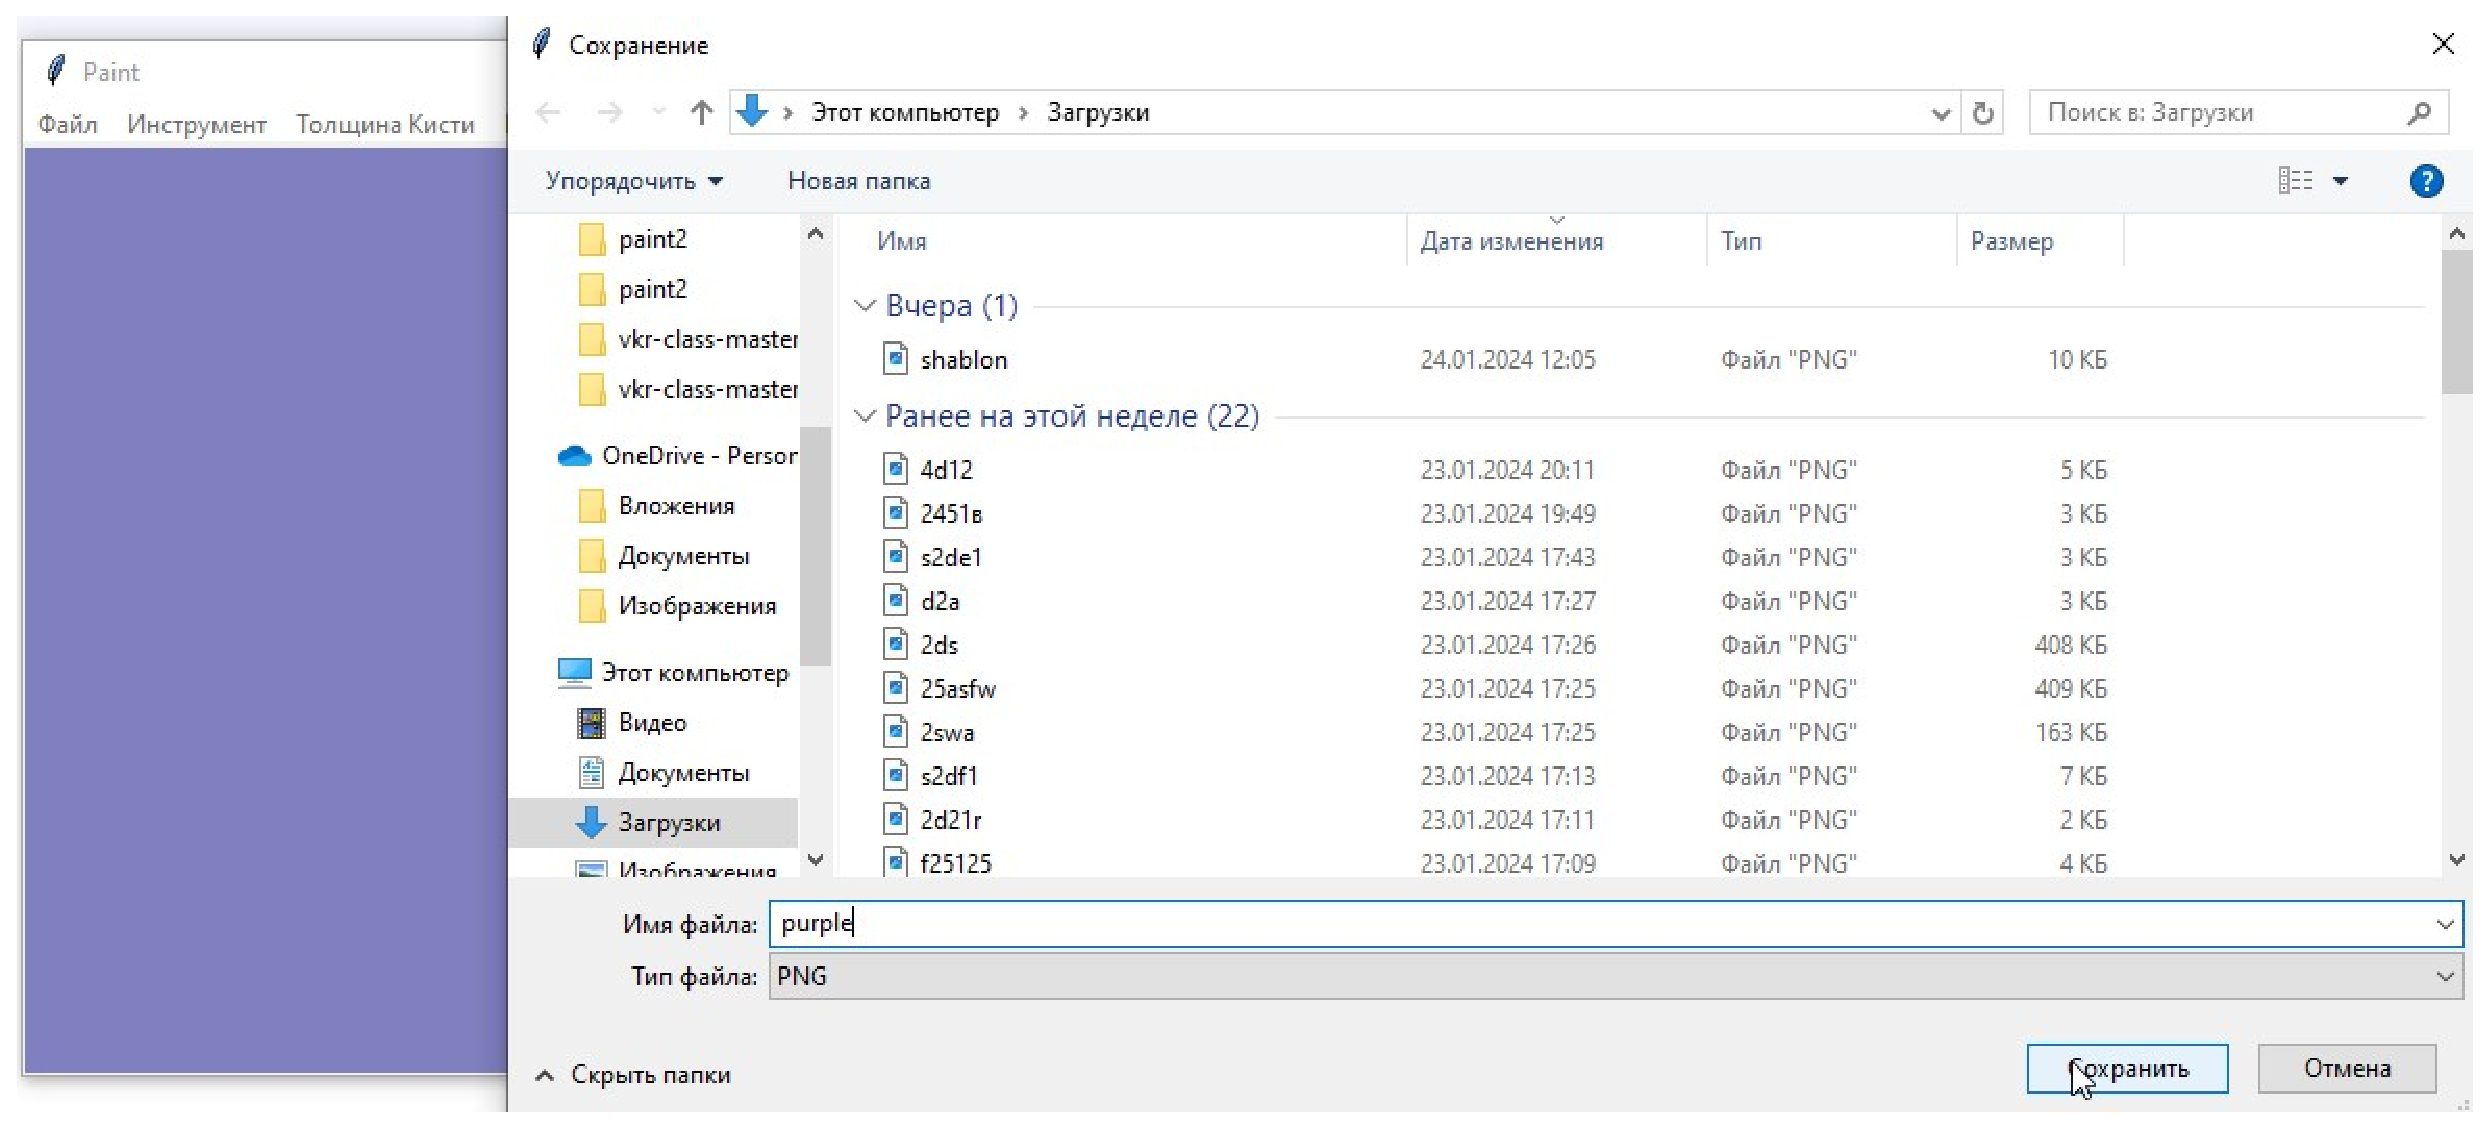
\includegraphics[width=1\linewidth]{sve}}
\caption{Сохранение файла}
\label{sve:image}
\end{figure}

На рисунке \ref{ope:image} представлено открытие файла через диалоговое окно.

\begin{figure}[H]
	\center{\includegraphics[width=1\linewidth]{ope}}
	\caption{Открытие файла}
	\label{ope:image}
\end{figure}

На рисунке \ref{size:image} представлено изменение размера кисти пользователем.

\begin{figure}[H]
	\center{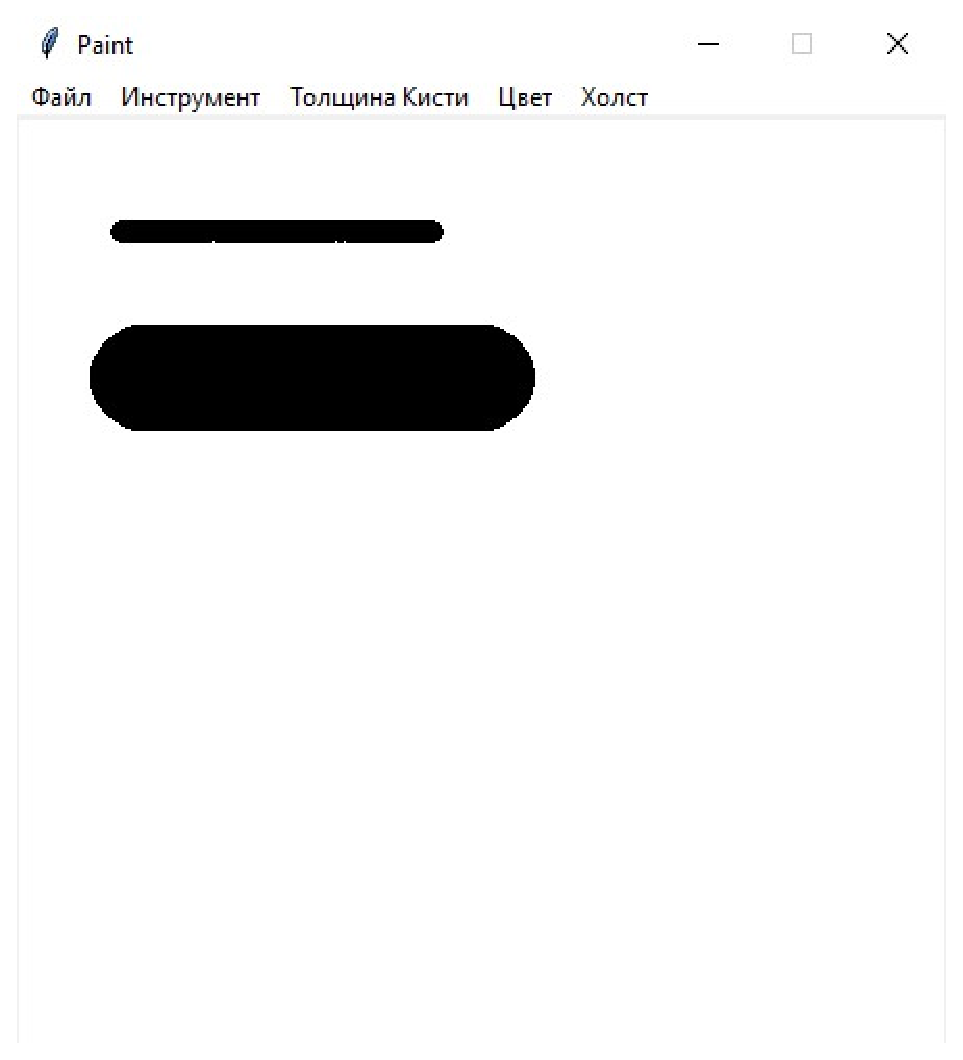
\includegraphics[width=1\linewidth]{size}}
	\caption{Изменение размера кисти}
	\label{size:image}
\end{figure}

На рисунке \ref{clr:image} представлено изменение цвета кисти пользователем.

\begin{figure}[H]
	\center{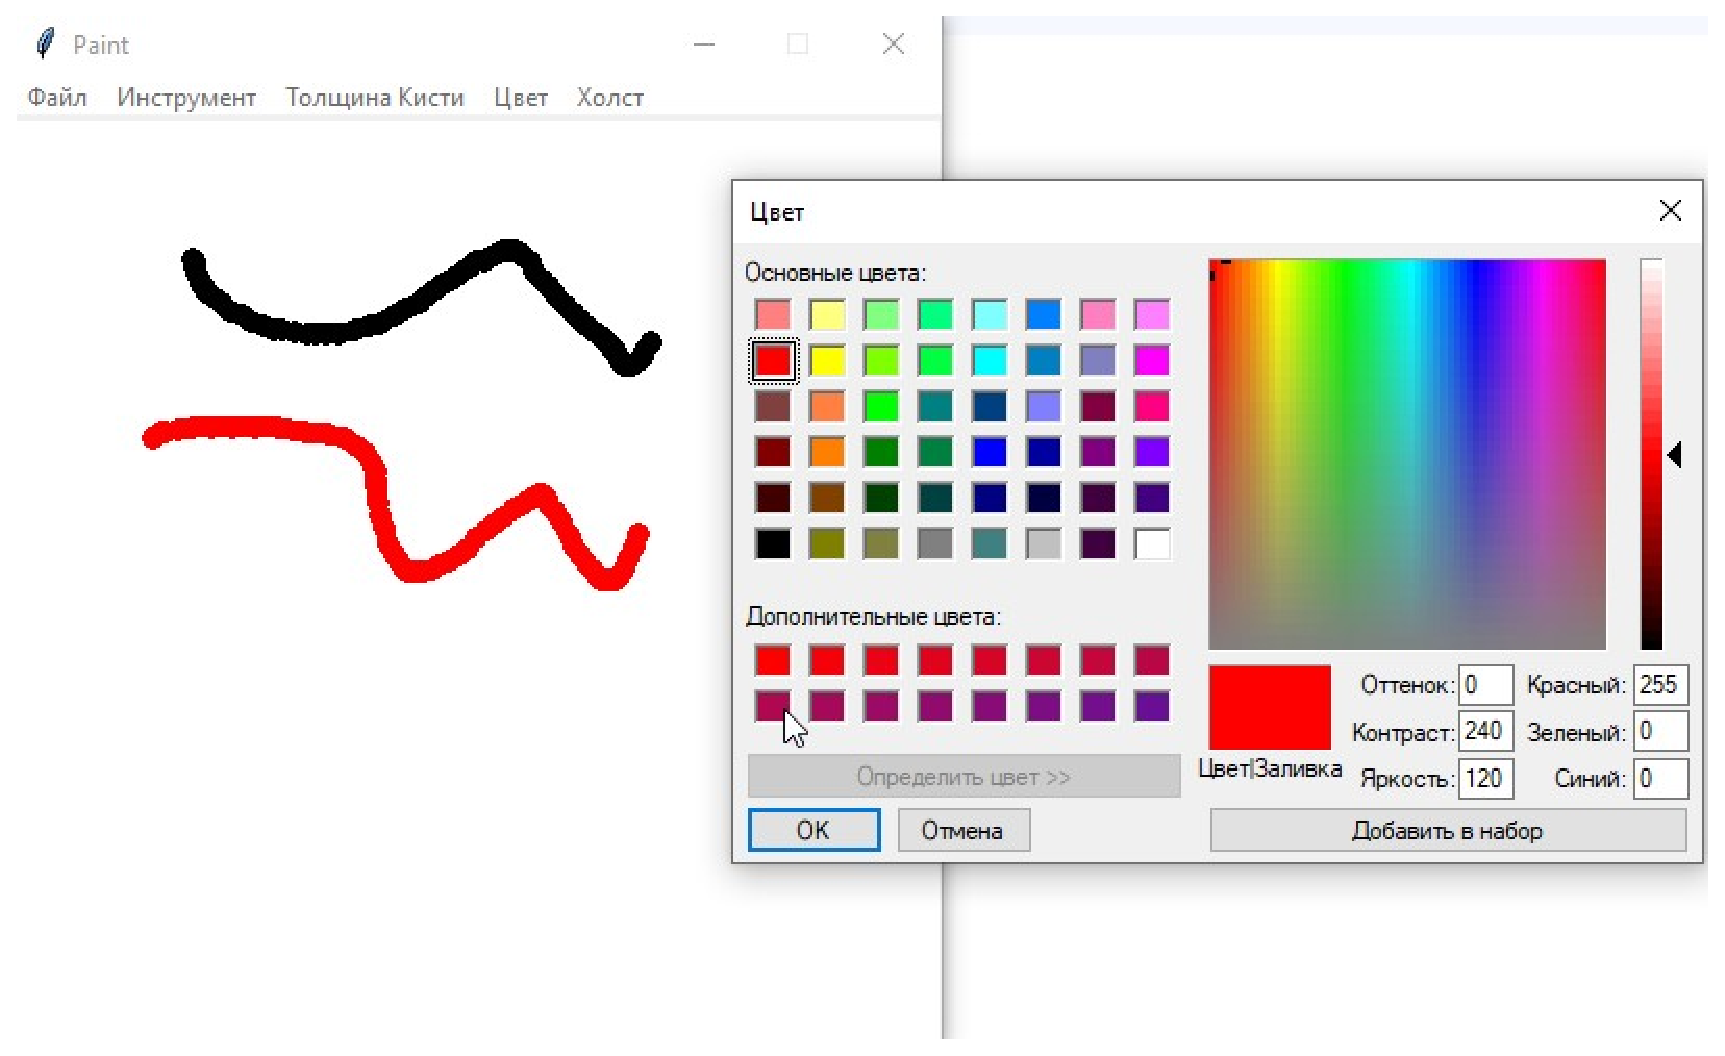
\includegraphics[width=1\linewidth]{clr}}
	\caption{Изменение цвета кисти}
	\label{clr:image}
\end{figure}

На рисунке \ref{hlst:image} представлена заливка всей рабочей зоны определенным цветом.

\begin{figure}[H]
	\center{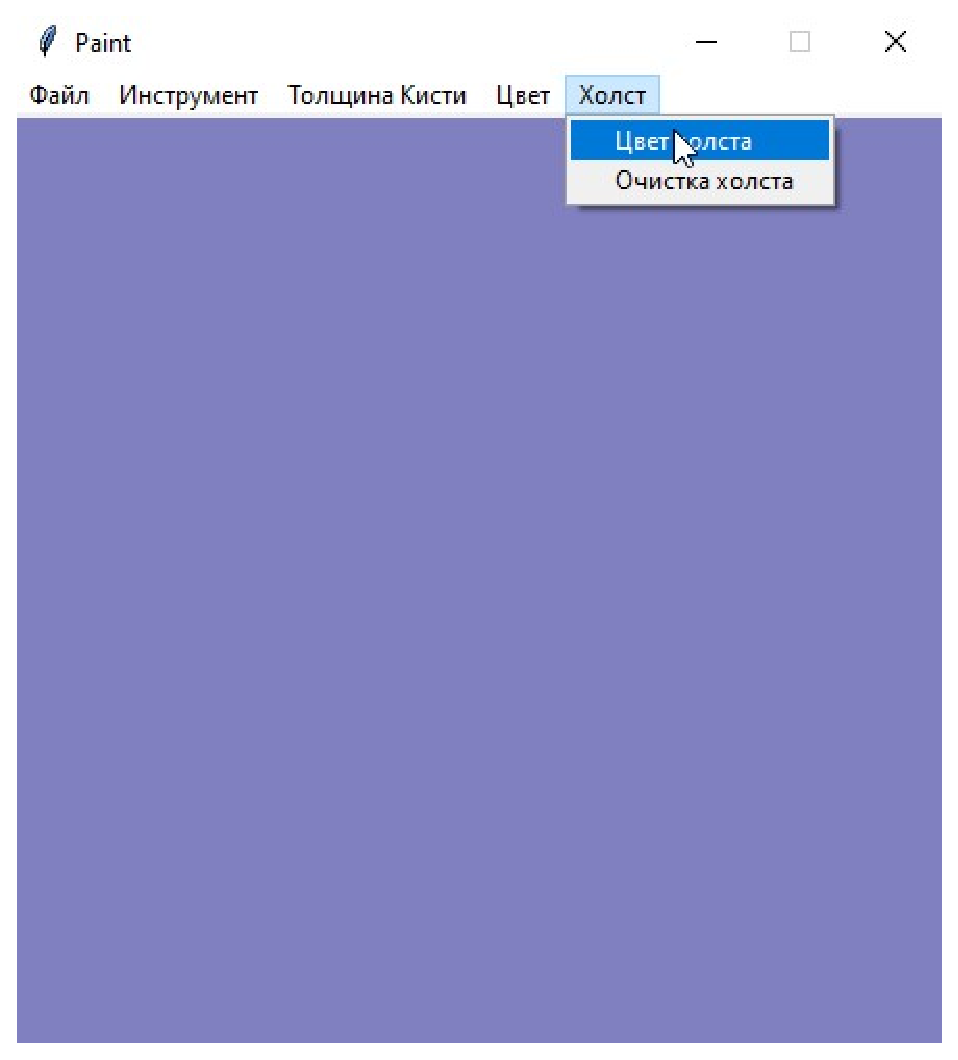
\includegraphics[width=1\linewidth]{hlst}}
	\caption{Заливка холста}
	\label{hlst:image}
\end{figure}
